%%%%%%%%%%%%%%%%%%%%%%%%%%%%%%%%%%%%%%%%%%%%%%%%%%%%%%%%%%%%%%%%%%%%%%%%%%%%%%
% CS114: Introduction to Programming in Java
% Copyright 2015 Pejman Ghorbanzade <mail@ghorbanzade.com>
% Creative Commons Attribution-ShareAlike 4.0 International License
% https://github.com/ghorbanzade/UMB-CS114-2015F/blob/master/LICENSE
%%%%%%%%%%%%%%%%%%%%%%%%%%%%%%%%%%%%%%%%%%%%%%%%%%%%%%%%%%%%%%%%%%%%%%%%%%%%%%

\def \topDirectory {../..}
\def \texDirectory {\topDirectory/src/main/tex}

\documentclass[compress]{beamer}
%\mode<presentation>
%\usetheme{default}

\usepackage{\texDirectory/template/style/directives}
%%%%%%%%%%%%%%%%%%%%%%%%%%%%%%%%%%%%%%%%%%%%%%%%%%%%%%%%%%%%%%%%%%%%%%%%%%%%%%
% CS114: Introduction to Programming in Java
% Copyright 2015 Pejman Ghorbanzade <mail@ghorbanzade.com>
% Creative Commons Attribution-ShareAlike 4.0 International License
% https://github.com/ghorbanzade/UMB-CS114-2015F/blob/master/LICENSE
%%%%%%%%%%%%%%%%%%%%%%%%%%%%%%%%%%%%%%%%%%%%%%%%%%%%%%%%%%%%%%%%%%%%%%%%%%%%%%

\course{id}{CS240}
\course{name}{Programming in C}
\course{venue}{Mon/Wed, 5:30 PM - 6:45 PM}
\course{semester}{Spring 2016}
\course{department}{Department of Computer Science}
\course{university}{University of Massachusetts Boston}

\instructor{name}{Pejman Ghorbanzade}
\instructor{title}{}
\instructor{position}{Student Instructor}
\instructor{email}{pejman@cs.umb.edu}
\instructor{phone}{617-287-6419}
\instructor{office}{S-3-124B}
\instructor{office-hours}{Mon/Wed 16:00-17:30}
\instructor{address}{University of Massachusetts Boston, 100 Morrissey Blvd., Boston, MA}

\usepackage{\texDirectory/template/style/beamerthemePejman}
\doc{number}{5}
%\setbeamertemplate{footline}[text line]{}

\usepackage{booktabs}
\usepackage{graphics}

\begin{document}

\prepareCover

\section{Operators}

\begin{slide}
	\begin{block}{Definition}

	An operation is an action performed on one or more values either to modify the value or to produce a new one.

	\end{block}
\end{slide}

\begin{slide}
	\begin{block}{Arithmetic Operators}

	\begin{columns}
	\column{0.4\textwidth}

	\begin{terminal}
	int a = 10;
	int b = 25;
	\end{terminal}

	\column{0.6\textwidth}
	\begin{table}
	\resizebox{\columnwidth}{!}{
	\begin{tabular}{lcc}
	\toprule
	Opeartor & Example & Output \\
	\midrule
	addition & \texttt{a + b} & 35 \\
	subtraction & \texttt{a - b} & -15 \\
	multiplication & \texttt{a * b} & 250 \\
	division & \texttt{b / a} & 2 \\
	modulus & \texttt{b \% a} & 5 \\
	\bottomrule
	\end{tabular}
	}
	\end{table}
	\end{columns}

	\end{block}
\end{slide}

\begin{slide}
	\begin{block}{Quiz}

	What is the final value of variables \texttt{d} and \texttt{e}?

	\begin{terminal}
	char c = 'a';
	int d = c + 3;
	char e = d + 1;
	\end{terminal}

	\end{block}

	\pause

	\begin{block}{Answer}

	\begin{terminal}
	printf("%d", c); // prints: 97
	printf("%d", d); // prints: 100
	printf("%c", e); // prints: 'e'
	\end{terminal}

	\end{block}
\end{slide}

\begin{slide}
	\begin{block}{Relational Operators}

	\begin{columns}
	\column{0.4\textwidth}

	\begin{terminal}
	int a = 99;
	int b = 100;
	char c = 'c';
	char d = 'd';
	\end{terminal}

	\column{0.6\textwidth}
	\begin{table}
	\resizebox{\columnwidth}{!}{
	\begin{tabular}{lcc}
	\toprule
	Operation & Example & Output \\
	\midrule
	greater than & \texttt{a > b} & 0 \\
	less than & \texttt{a < b} & 1 \\
	greater than or equal to & \texttt{a >= c} & 1 \\
	less than or equal to & \texttt{b <= d} & 1 \\
	equal to & \texttt{a == c} & 1 \\
	not equal to & \texttt{b != d} & 0 \\
	\bottomrule
	\end{tabular}
	}
	\end{table}
	\end{columns}

	\end{block}
\end{slide}

\begin{slide}
	\begin{block}{Logical Operators}

	\begin{columns}
	\column{0.4\textwidth}

	\begin{terminal}
	int a = 99;
	int b = 100;
	char c = 'c';
	char d = 'd';
	\end{terminal}

	\column{0.6\textwidth}
	\begin{table}
	\resizebox{\columnwidth}{!}{
	\begin{tabular}{lcc}
	\toprule
	Operation & Example & Output \\
	\midrule
	logical AND & \texttt{a < c \&\& a < d} & 0 \\
	logical OR & \texttt{a < b || a < c} & 1 \\
	logical NOT & \texttt{!(a < b)} & 0 \\
	\bottomrule
	\end{tabular}
	}
	\end{table}
	\end{columns}

	Expressions connected by logical operators are evaluated from left to right. Evaluation terminates once the final value is determined.

	\end{block}
\end{slide}

\begin{slide}
	\begin{block}{increment and decrement operators}

	\begin{columns}
	\column{0.4\textwidth}

	\begin{terminal}
	int a = 1;
	\end{terminal}

	\column{0.6\textwidth}
	\begin{table}
	\resizebox{\columnwidth}{!}{
	\begin{tabular}{lcc}
	\toprule
	Operation & Example & Output \\
	\midrule
	increment & \texttt{a++} & 2 \\
	increment & \texttt{++a} & 2 \\
	decrement & \texttt{a--} & 0 \\
	decrement & \texttt{--a} & 0 \\
	\bottomrule
	\end{tabular}
	}
	\end{table}
	\end{columns}

	\end{block}
\end{slide}

\begin{slide}
	\begin{block}{Quiz}

	What is the output of the following code snippet?

	\begin{terminal}
	int a = 1;
	int b = 2;
	if (++a && a == b)
	    printf("Programming");
	if (b++ == a)
	    printf(" is fun");
	\end{terminal}

	\end{block}
\end{slide}

\begin{slide}
	\begin{block}{Bitwise Operators}

	\begin{columns}
	\column{0.45\textwidth}
	\begin{terminal}
	int a = 0b11110000;
	int b = 0b10101010;
	\end{terminal}

	\column{0.55\textwidth}
	\begin{table}
	\resizebox{\columnwidth}{!}{
	\begin{tabular}{lcc}
	\toprule
	Operation & Example & Output \\
	\midrule
	bitwise AND & \texttt{a \& b} & 0b10100000 \\
	bitwise inclusive OR & \texttt{a | b} & 0b11111010 \\
	bitwise exclusive OR & \texttt{a \^{} b} & 0b01011010 \\
	left binary shift & \texttt{a << 1} & 0b11100000 \\
	right binary shift & \texttt{a >> 1} & 0b01111000 \\
	one's complement & \texttt{\~{}a} & 0b00001111 \\
	\bottomrule
	\end{tabular}
	}
	\end{table}
	\end{columns}

	\end{block}
\end{slide}

\begin{slide}
	\begin{block}{Assignment Operators}

	An assignment operator (\alert{\texttt{=}}) stores a new value into a variable.

	Assignment statements such as ${exp}_1 = {exp}_1 {op} {exp}_2$ can equivalently be written as ${exp}_1 {op}= {exp}_2$ where ${op}$ is one of the following operators:

	\texttt{+}\hfill \texttt{-}\hfill \texttt{*}\hfill \texttt{/}\hfill \texttt{\%}\hfill \texttt{<<}\hfill \texttt{>>}\hfill \texttt{\&}\hfill \texttt{\^{}}\hfill \texttt{|}

	An assignment statement has a value and can occur in expressions.

	\end{block}
\end{slide}

\section{Conditionals}

\begin{slide}
	\begin{block}{Statements}

	A statement is the smallest standalone element that provide a meaningful machine instruction. A statement is terminated by a semicolon.

	Function of a program is determined based on the set of statements in its \texttt{main} function executed in succession.
	A program terminates once all statements in its \texttt{main} function are executed.

	\end{block}
\end{slide}

\begin{slide}
	\begin{block}{\texttt{if} statement}

	An \texttt{if} statement contains an expression followed by a block of statements.
	Statements within the block are executed if the value of expression is evaluated to non-zero.

	\begin{terminal}
	if (@*\textit{expression}*@) {
	    @*$\mathit{statement}_1$*@;
	    @*$\mathit{statement}_2$*@;
	}
	\end{terminal}

	\end{block}
\end{slide}

\begin{slide}
	\begin{block}{Coding Style Convention}

	\begin{terminal}
	if (number_statements > 1) {
	    printf("MUST");
	    printf("preserve braces");
	}
	if (number_statements == 1)
	    printf("remove braces");
	if (number_statements == 0);
	\end{terminal}

	\end{block}
\end{slide}

\begin{slide}
	\begin{block}{Coding Style Convention}

	\begin{terminal}
	int a = 2;
	if (a != 0)
	    printf("Hello");
	\end{terminal}

	It is often recommended to avoid redundancy in expressions.

	\begin{terminal}
	int a = 2;
	if (a)
	    printf("Hello");
	\end{terminal}

	\end{block}
\end{slide}

\begin{slide}
	\begin{block}{\texttt{if-else} statement}

	\begin{terminal}
	int a = 2;
	if (a == 2)
	    printf("Hello");
	else
	    printf("Can you hear me?");
	\end{terminal}

	\end{block}
\end{slide}

\begin{slide}
	\begin{block}{\texttt{if-else-if} statement}

	\begin{terminal}
	int a = 3;
	if (a == 1)
	    printf("Hello");
	else if (a == 2)
	    printf("Can you hear me?");
	else
	    printf("How are you?");
	\end{terminal}

	\end{block}
\end{slide}

\begin{slide}
	\begin{block}{Coding Style Convention}

	Braces should be used for all branches if at least one of them contains more than one statement.

	\begin{terminal}
	int a = 3;
	if (a == 1) {
	    printf("Hello");
	} else {
	    printf("How are you?");
	    printf("Can you hear me?);
	}
	\end{terminal}

	\end{block}
\end{slide}

\begin{slide}
	\begin{block}{\texttt{switch} statement}

	The \texttt{switch} statement is a multi-way decision that tests whether an expression matches one of a number of \alert{constant} integer values, and branches accordingly.

	\begin{terminal}
	switch (@*\textit{expression}*@) {
	case @*$\mathit{val}_1$*@:
	    statements;
	case @*$\mathit{val}_2$*@:
	    @*\textit{statements}*@;
	default:
	    @*\textit{statements}*@;
	}
	\end{terminal}

	\end{block}
\end{slide}

\section{Loops}

\begin{slide}
	\begin{block}{\texttt{while} statement}

	A \texttt{while} statement contains an expression followed by a block of statements.

	Statements within the block are executed \emph{as long as} the value of expression is evaluated to non-zero.

	\begin{terminal}
	while (@*\textit{expression}*@) {
	    @*\textit{statements}*@;
	}
	\end{terminal}

	\end{block}
\end{slide}

\begin{slide}
	\begin{block}{\texttt{do-while} statement}

	A \texttt{do-while} statement is a \texttt{while} loop whose expression is evaluated after execution of its block of statements.

	\begin{terminal}
	do {
	    @*\textit{statements}*@;
	} while (@*\textit{expression}*@);
	\end{terminal}

	\end{block}
\end{slide}

\begin{slide}
	\begin{block}{\texttt{for} statement}

	A \texttt{for} statement contains three expressions followed by a block of statements.

	\begin{itemize}
	\item[] $\mathit{exp}_1$ pre-loop expression
	\item[] $\mathit{exp}_2$ iteration condition
	\item[] $\mathit{exp}_3$ post-iteration expression
	\end{itemize}

	\begin{terminal}
	for (@*$\mathit{exp}_1$*@; @*$\mathit{exp}_2$*@; @*$\mathit{exp}_3$*@) {
	    @*\textit{statements}*@;
	}
	\end{terminal}

	\end{block}
\end{slide}

\begin{slide}
	\begin{block}{Remember}

	\begin{itemize}
	\item[] A \texttt{for} statement is often used when the number of loop iterations is already known.
	\item[] Mastering the \texttt{while} statement can boost your code quality.
	\end{itemize}

	\begin{terminal}
	int i = 0;
	while ((ch = str[i++]) != '\0');
	printf("length of str: %d\n", i);
	\end{terminal}

	\end{block}
\end{slide}

\begin{slide}
	\begin{block}{Infinite Loops}

	\begin{terminal}
	for (;;) {
	    @*\textit{statements}*@;
	}
	\end{terminal}

	\begin{terminal}
	while (1) {
	    @*\textit{statements}*@;
	}
	\end{terminal}

	An infinite \texttt{while} loop is often preferred for its superior readability.

	\end{block}
\end{slide}

\begin{slide}
	\begin{figure}
	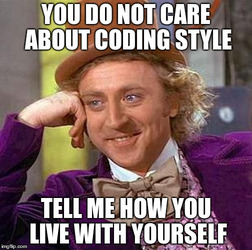
\includegraphics[width=0.5\textwidth]{\texDirectory/img/wonka.jpg}
	\end{figure}
\end{slide}

\section{Unconditional Branches}

\begin{slide}
	\begin{block}{Definition}

	Unconditional branches are statements that change program control flow without the need to evaluate an expression.

	Bohm-Jacopini theorem states that any computing application can be realized without the use of Unconditional branches.

	\end{block}
\end{slide}

\begin{slide}
	\begin{block}{\texttt{break} statement}

	A \texttt{break} statement immediately terminates the loop regardless of its iteration condition and moves program control flow to the next statement after the loop.

	\begin{terminal}
	int i = 2;
	int num = 25;
	int prime = 0;
	while (i <= num / 2)
	    if (num % i == 0) {
	        prime = 1;
	        break;
	    }
	\end{terminal}

	\end{block}
\end{slide}

\begin{slide}
	\begin{block}{\texttt{continue} statement}

	A \texttt{continue} statement skips the remaining statements of the loop and moves program control flow to the next iteration of the loop.

	\begin{terminal}
	int i = 2;
	int num = 25;
	int prime = 0;
	while (i <= num / 2) {
	    if (num % i)
	        continue;
	    prime = 1;
	}
	\end{terminal}

	\end{block}
\end{slide}

\begin{slide}
	\begin{block}{\texttt{goto} statement}

	A \texttt{goto} statement changes program control flow to the label it points to.
	\begin{terminal}
	    a = 2;
	    if (a == 2)
	        goto ERROR;
	    printf("Hello");

	ERROR:
	    printf("Goodbye");
	\end{terminal}

	\end{block}
\end{slide}

\begin{slide}
	\begin{block}{Labels}

	A label is simply a name for a certain point in the program control flow that may be referred to by a \texttt{goto statement}.

	\begin{terminal}
	    a = 2;
	    if (a == 2)
	        goto ERROR;
	    printf("Hello");

	ERROR:
	    printf("Goodbye");
	\end{terminal}

	\end{block}
\end{slide}

\begin{slide}
	\begin{quotation} \scriptsize \normalfont

	C provides the infinitely-abusable \texttt{goto} statement and labels to branch to.
	[...]
	There are a few situations where \texttt{goto}s may find a place such as breaking out of two or more loops at once.

	Code involving a \texttt{goto} can always be written without one, though perhaps at the price of some repeated tests or an extra variable.
	[...]
	With a few exceptions code that relies on \texttt{goto} statements is generally harder to understand and to maintain than code without \texttt{goto}s.
	Although we are not dogmatic about the matter, it does seem that \texttt{goto} statements should be used rarely, if at all.

	\begin{flushright}-- The C Programming Language (K\&R)\end{flushright}

	\end{quotation}
\end{slide}

\begin{slide}
	\begin{quotation} \scriptsize \normalfont

	Albeit deprecated by some people, the equivalent of the \texttt{goto} statement is used frequently by compilers in form of the unconditional jump instruction.

	The \texttt{goto} statement comes in handy when a function exits from multiple locations and some common work such as cleanup has to be done.
	If there is no cleanup needed then just return directly.

	The rationale for using \texttt{goto}s is:
	(1) Unconditional statements are easier to understand and follow.
	(2) Nesting is reduced.
	(3) Errors by not updating individual exit points when making modifications are prevented.
	(4) Unconditional statements save the compiler work to optimize redundant code away.

	\begin{flushright}-- Linux Kernel Coding Style\end{flushright}

	\end{quotation}
\end{slide}

\end{document}
